%!TEX root = ../these.tex

\section{Технологические ограничения современных машин листовой резки с ЧПУ}
\label{sec:cut.constr}

Полученный любым способом маршрут движения режущего инструмента~
\eqref{eq:cut.tuple},
должен быть исполнен на конкретном промышленном оборудовании ---
режущей машине с ЧПУ.
Это накладывает ряд существенных ограничений на решение задачи резки,
в терминах формулы \eqref{eq:cut.problem} ---
существенно ограничивает проблемное пространство
$\mathfrak G$.
Рассмотрим некоторые из этих ограничений.

\subsection{Позиции точек врезки и выключения инструмента}
\label{sec:cut.area}

Это естественно возникающие технологические ограничения,
которые естественно называть <<геометрическими>>,
вызваны тем,
что, как сказано выше,
точка врезки должна располагаться на некотором
ненулевом расстоянии от контура детали.
Кроме того, они не должны попадать внутрь других деталей,
с учетом припуска на ширину реза.
Конкретные расстояния определяются используемыми технологиями.

Введем обозначения:
эквидистанты замкнутых контуров
$C_1, C_2, \dots C_N$,
удаленные от них на расстояние $d$,
обозначим за
$C_1^{+d}, C_2^{+d}, \dots C_N^{+d}$,
а ограниченные этими эквидистантами
двумерные геометрические объекты ---
$\widetilde C_1^{+d}, \widetilde C_2^{+d}, \dots \widetilde C_N^{+d}$,
$\widetilde C_i^{+d} \in \mathbb R \times \mathbb R$.
Для внешних контуров берется внешняя эквидистанта,
для внутренних --- соответственно внутренняя.
Далее, пусть
$OUT = \{i_1^+, i_2^+, \dots i_{N^+}^+\} \subseteq \overline{1, N}$ ---
множество индексов внешних контуров,
а
$IN = \{i_1^-, i_2^-, \dots i_{N^-}^-\} \subset \overline{1, N}$ ---
множество индексов внутренних,
$|OUT|=N^+$,
$|IN|=N^-$,
если внутренних контуров на раскройной карте нет,
то $N^+=N$, $N^-=0$, $IN=\varnothing$.

Если минимальное расстояние от контура детали до точки врезки
$d_1$,
то позиции точек врезки должны удовлетворять условию
$M_i \in G_M, \forall i \in \overline{1, N}$,
где
\begin{equation}
  \label{eq:cut.pierce}
  G_M = \left(\mathcal B \setminus \bigcup_{i \in OUT} \widetilde C_i^{+d_1} \right)
  \cup \bigcup_{i \in IN} \widetilde C_i^{+d_1}
\end{equation}

Аналогично может быть записано ограничение для
позиций точек выключения инструмента
$M^*_i \in G_{M^*}, \forall i \in \overline{1, N}$:
\begin{equation}
  \label{eq:cut.off}
  G_{M^*} = \left(\mathcal B \setminus \bigcup_{i \in OUT} \widetilde C_i^{+d_2} \right)
  \cup \bigcup_{i \in IN} \widetilde C_i^{+d_2}
  ,
\end{equation}
где
$d_2$ --- допустимое расстояние
от контуров деталей до точек выключения инструмента;
как правило
$0 \leqslant d_2 < d_1$.

\begin{figure}
  \centering
  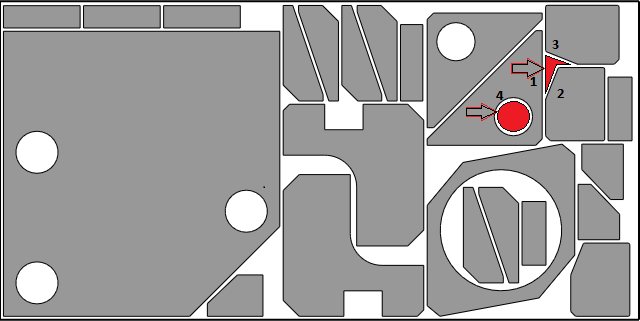
\includegraphics[width=0.9\textwidth]{pierce-area.png}
  \caption{
    Пример двух геометрических областей на раскройной карте,
    допустимых для задания точек врезки
  }
  \label{fig:cut.pierce-area}
\end{figure}

На рис.~\ref{fig:cut.pierce-area}
показаны стрелками и выделены цветом
две геометрические области листа,
одна, определяемая
внешними граничными контурами деталей,
обозначенных цифрами
\textit{1, 2} и \textit{3},
и вторая ---
внутренним граничным контуром
\textit{4}.
Минимально допустимое расстояние
от граничных контуров
\textit{1--4} до возможных точек врезки
$d_1=9.5$~мм.

\subsection{Условия предшествования}
\label{sec:cut.PC}

Это одно из самых <<популярных>>
технологических ограничений на элементы
маршрута~\eqref{eq:cut.tuple},
оно обусловлено особенностями машин портального типа
~\cite{bi:Petunin2,bi:dewil-review,bi:Dewil2015}.
После вырезания замкнутого контура,
его внутренняя часть ничем не удерживается и может сдвигаться,
поворачиваться, наклоняться или даже падать.
В некоторых случаях возможно столкновение
режущей головки и заготовки с повреждением дорогостоящего инструмента.
Во избежание этого, следует придерживаться следующих правил:
\begin{enumerate}
  \item
  Если внешний контур содержит один или более внутренних контуров,
  которые представляют собой границы отверстий в деталях,
  то прежде, чем будет начата вырезка внешнего контура,
  должны быть вырезаны все
  внутренние контуры.
  \item
  Если внутренний контур детали на раскройной карте содержит внешний контур/контуры другой детали,
  то сначала должна быть вырезана эта другая деталь с соблюдением предыдущего пункта.
\end{enumerate}

Эти правила и называются \textit{условиями предшествования}
для перестановки
$ I = (i_1, i_2, \,\dots, i_K)$.
В терминах ее элементов условие означает следующее:
\begin{itemize}
  \item
  если в перестановке
  $ I = (i_1, i_2, \,\dots, i_K)$
  сегмент $i_k$
  содержит внешний контур,
  то все соответствующие внутренние контуры должны содержаться в сегментах,
  предшествующих сегменту $i_k$
  в перестановке;
  \item
  если в перестановке
  $ I = (i_1, i_2, \,\dots, i_K)$
  сегмент $i_k$
  содержит  внутренний контур,
  который на раскройной карте содержит внутри внешний контур,
  соответствующий другому объекту
  $A_l$
  $(l=1,2, \,\dots, n)$,
  то этот внешний контур должен быть вырезан в сегментах,
  предшествующих сегменту $i_k$ в перестановке $I$.
\end{itemize}

Таким образом,
ограничения предшествования ограничивают
множество допустимых перестановок
$ I = (i_1, i_2, \,\dots, i_K)$
в маршруте $\mathfrak R$
и могут называться
\textit{комбинаторными}
или дискретными ограничениями.
Следует отметить,
что они
(так же, как ограничения
предыдущего раздела~\ref{sec:cut.area})
однозначно вычисляются по раскройной карте
и не зависят от других элементов кортежа~
\eqref{eq:cut.tuple}.

\subsection{Эвристические правила термической резки заготовок
из листовых материалов}

В отличие от вышеописанных,
следующий тип технологических требований накладывает условия на
выбор точки врезки и порядка резки сегментов в зависимости от того,
какие параметры маршрута резки были выбраны на предыдущих шагах.
Этот тип ограничений обусловлен геометрическими искажениями материала
в процессе термической резки деталей.
Эти правила разработаны сотрудниками ОАО <<Уралхиммаш>>
В.И.~Кротовым и А.Д.~Гуртовенко
на основе опыта резки листовых материалов на машинах термической резки с~ЧПУ
в~котельно-заготовительном комплексе предприятия.

Термические воздействия на вырезаемые заготовки можно подразделить на два типа:
\begin{itemize}
\item
общие изменения геометрических размеров заготовки (уменьшение)
вследствие ее вырезания из нагретой части материала;
\item
изменение геометрической формы заготовок
(изменение радиусов у секторов,
отклонения от прямолинейности у прямоугольных деталей) и др.
Чем больше геометрические размеры заготовки,
тем больше изменения.
Наиболее  подвержены изменениям узкие длинные заготовки.
\end{itemize}

На величину термических деформаций оказывают влияние:
\begin{itemize}
\item	тип резки: газовая, плазменная, лазерная, \dots
\item	марка материала, его теплопроводность;
\item	состояние поставки металла (наличие внутренних напряжений), его термообработка;
\item	толщина металла;
\item	выбор порядка резки заготовок;
\item	выбор точек врезки для каждого контура;
\item	направление обхода контура (по/против часовой стрелки).
\item и т.п.
\end{itemize}

Наиболее важные из технологических требований резки,
обусловленные наличием термических деформаций материала,
сформулированы в виде двух правил ---
<<жесткости заготовки / детали>> и <<жесткости листа / материала>>,
см.~\cite{Sozopol,Miskolc}.

\subsubsection{Правило <<жесткости детали>>}
При резке контура точка
врезки и направление резки контура выбираются таким образом,
чтобы сначала вырезались участки контура,
расположенные в непосредственной близости к границе материала,
либо к границе вырезанной области,
а завершение резки происходило по участку контура,
граничащего с <<жесткой>> (не вырезанной) частью области.

Важно отметить,
что при изменении порядка вырезки заготовок
(например, в последовательности сверху вниз)
изменится и набор допустимых точек врезки и направлений реза.

\subsubsection{Правило <<жесткости листа>>}

Это правило накладывает ограничение на
последовательность
$i_1, i_2, \,\dots, i_k$,
то есть порядок,
в котором вырезаются используемые сегменты резки
$S_1, S_2, \,\dots, S_K$.
Фактически оно состоит из нескольких
эмпирических условий.

\begin{itemize}
  \item
  Если
  среди заготовок имеются длинномерные детали
  (один из габаритов больше другого в $\approx 10$ раз и более)
  и они расположены вблизи
  узкой границы материала,
  то процесс резки следует начинать с них,
  так как именно такого рода заготовки
  подвержены максимальным тепловым деформациям.
  \item
  Если на материале есть крупный отход,
  то
  процесс резки следует начать с противоположной стороны,
  поскольку аккумулирующееся в материале в~процессе резки
  тепло в конечной стадии резки должно быть
  несколько скомпенсировано <<жестким>> остатком.
  \item
  Иначе
  резку следует начинать с той стороны,
  где суммарные тепловыделения от резки больше
  (больше мелких деталей, либо больше суммарный периметр реза).
  \item
  При выборе последовательности вырезаемых заготовок
  на материале не должно оставаться узких полос и <<островов>>,
  содержащих не вырезанные заготовки.
\end{itemize}

Следует отметить, что, как показала практика,
правила <<жесткости заготовки>> и <<жесткости материала>>
целесообразно учитывать
не только при разработке управляющих программ для машин газовой,
плазменной и лазерной резки с ЧПУ,
но и при применении машин гидроабразивной фигурной листовой резки.
Этот факт свидетельствует о том,
что изменения геометрических характеристик материала
связаны не только с термическими деформациями,
но и с механическими трансформациями материала
при листовой резке заготовок на машинах с ЧПУ,
см.~\cite{bi:book2020}.

Вопросы математической формализации ограничений,
связанных именно с технологическими требованиями термической резки,
все еще остаются наименее изученными.

Если обозначить через
$\mathfrak R_\nu$
частичный маршрут резки первых $\nu$
сегментов
($\nu < K$)
$$
  \mathfrak R_\nu = \left<
    M_0, M_1, S_1, M_1^*, \,\dots, M_\nu, S_\nu, M_\nu^*,
    i_1, i_2, \,\dots, i_\nu
  \right>
  ,
$$
то правила <<жесткости заготовки>> и <<жесткости материала>>
при формировании допустимого маршрута
$\mathfrak R$,
помимо соблюдения условий предшествования для перестановки
$i_1, i_2, \,\dots, i_K$
и условий \eqref{eq:cut.pierce} и \eqref{eq:cut.off},
формирует следующее дополнительное условие:
если
$\mathfrak R_\nu$ -- частичный маршрут,
допустимый с точки зрения всех технологических
требований листовой резки,
сформулированных в этом параграфе,
то сегмент с номером $(\nu+1)$
и соответствующая точка врезки $M_{(\nu+1)}$
для него в маршруте
$\mathfrak R_{(\nu+1)}$
должны выбираться с учетом уже выбранного частичного маршрута
$\mathfrak R_\nu$,
что фактически означает либо запрет
на некоторые <<плохие>> номера сегментов
$i_{(\nu+1)}$
и <<плохие>> точки врезки
$M_{(\nu+1)}$
в области  $G_M$,
либо наложение <<штрафа>> на <<плохие>> значения
этих параметров кортежа
посредством включения наложенного штрафа в целевые функции
\eqref{eq:cut.time} -- \eqref{eq:cut.cost}
при решении оптимизационной задачи~\eqref{eq:cut.problem}.

Таким образом,
условия <<жесткости заготовки>> и <<жесткости материала>>
порождают для задачи непрерывно-дискретной оптимизации
своего рода \textit{динамические} ограничения,
формируемые только в процессе вычисления допустимого решения задачи.
